\documentclass{standalone}
\usepackage{pgfplots}
\pgfplotsset{compat=1.18}

\begin{document}

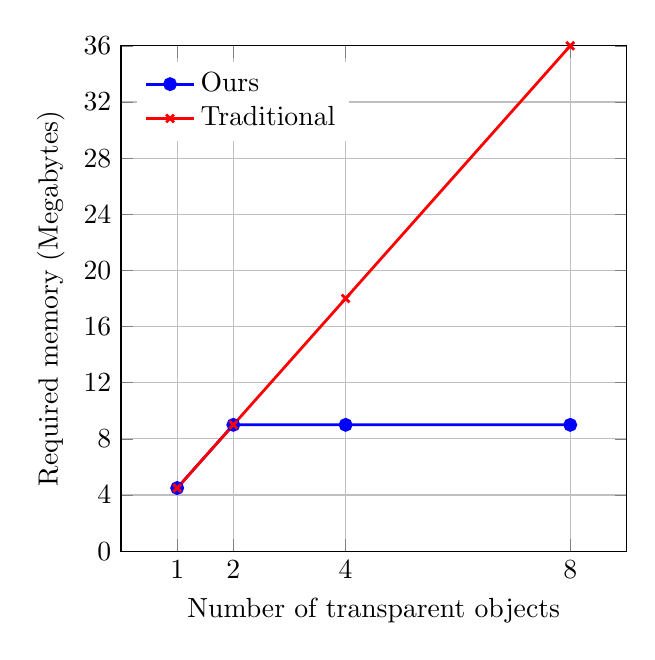
\begin{tikzpicture}
    \begin{axis}[
        width=8cm, height=8cm,
        xlabel={Number of transparent objects},
        ylabel={Required memory (Megabytes)},
        xmin=0, xmax=9,
        ymin=0, ymax=36,
        xtick={1,2,4,8},
        ytick={0,4,8,12,16,20,24,28,32,36},
        grid=both,
        legend pos=north west,
        legend cell align={left},
        legend style={draw=none}
    ]
    \addplot[
        color=blue,
        mark=*,
        line width=1pt
        ]
        coordinates {
        (1,4.5)(2,9)(4,9)(8,9)
        };
    \addplot[
        color=red,
        mark=x,
        line width=1pt
        ]
        coordinates {
        (1,4.5)(2,9)(4,18)(8,36)
        };
    \legend{Ours, Traditional}
    \end{axis}
\end{tikzpicture}

\end{document}